% ------------------------------------------------------------------------------
% LaTeX Template: Titlepage
% This is a title page template which be used for both articles and reports.
%
% Copyright: http://www.howtotex.com/
% Date: April 2011
% ------------------------------------------------------------------------------

% -------------------------------------------------------------------------------
% Preamble
% -------------------------------------------------------------------------------
\documentclass[paper=a4, fontsize=11pt,twoside]{scrartcl}		% Koma article

\usepackage[a4paper,pdftex]{geometry}										% A4paper margins
\setlength{\oddsidemargin}{5mm}												% Remove 'twosided' indentation
\setlength{\evensidemargin}{5mm}
\usepackage{graphicx}

\usepackage{fancyhdr} % Required for custom headers
\usepackage{lastpage} % Required to determine the last page for the footer
\usepackage{extramarks} % Required for headers and footers

\usepackage[english]{babel}
\usepackage[protrusion=true,expansion=true]{microtype}	
\usepackage{amsmath,amsfonts,amsthm,amssymb}
\usepackage{graphicx}
\usepackage[nottoc,numbib]{tocbibind} % Required for inlucde reference in TOC
\usepackage[pdfstartview=FitH,
CJKbookmarks=true,
bookmarksnumbered=true,
bookmarksopen=true,
colorlinks,
pdfborder=001,
linkcolor=black,
citecolor=blue,
]{hyperref} % Required for hyper link references

% ------------------------------------------------------------------------------
% Definitions (do not change this)
% ------------------------------------------------------------------------------
\newcommand{\HRule}[1]{\rule{\linewidth}{#1}} 	% Horizontal rule

\makeatletter							% Title
\def\printtitle{%						
    {\centering \@title\par}}
\makeatother									

\makeatletter							% Author
\def\printauthor{%					
    {\centering \large \@author}}				
\makeatother							

% ------------------------------------------------------------------------------
% Metadata (Change this)
% ------------------------------------------------------------------------------
\title{	\normalsize \textsc{Title page subtitle} 	% Subtitle of the document
		 	\\[2.0cm]													% 2cm spacing
			\HRule{0.5pt} \\										% Upper rule
			\LARGE \textbf{\uppercase{Interim Report}}	% Title
			\HRule{2pt} \\ [0.5cm]								% Lower rule + 0.5cm spacing
			\normalsize \today									% Todays date
		}

\author{
		\textbf{Group Id:} 5\\	
		\textbf{Group Member: } Zhefeng ZHOU\\  Yangyu GAO\\  Jiaying SUN\\ Zhe REN\\  Muyi JIANG\\  KAN LIU\\
		\textbf{Supervisor: } Heshan DU\\
        }
    
\begin{document}
% ------------------------------------------------------------------------------
% Maketitle
% ------------------------------------------------------------------------------
\thispagestyle{empty}				% Remove page numbering on this page
\printtitle									% Print the title data as defined above
  	\vfill
\printauthor								% Print the author data as defined above
\cleardoublepage

% ------------------------------------------------------------------------------
%  table of contents
% ------------------------------------------------------------------------------
\newpage
\tableofcontents
\thispagestyle{empty}	
\newpage
\cleardoublepage

% ------------------------------------------------------------------------------
% Begin document
% ------------------------------------------------------------------------------

\setcounter{page}{1}

% ------------------------------------------------------------------------------
% INTRODUCTION      Kan LIU
% ------------------------------------------------------------------------------
\section{Introduction}
\subsection{Description}
\subsection{Goal}
\subsection{Roles of member }


% ------------------------------------------------------------------------------
% Background Research   Kan LIU, Jiaying SUN, Zhe REN
% ------------------------------------------------------------------------------
\section{Background Research}
\subsection{Technical research}
% Ninja progess
For the main frame of the sorting algorithm animation, the interface is divided into 5 parts. Each of these 5 parts is not independent. 
\begin{enumerate}
	\item First, we did some research about different platforms. For PC platform, the advantage is that computer has more storage space then other device to install a software. It also has larger display screen, which can make animation, the main function of our designed software, seems more clear and visual. Therefore, we can design more functions for PC software developing. For mobile device, it is convenient for users to use the application whenever and wherever possible. The operating steps should also be easier than PC platform. For different operating system, we find a research from StatCounter Global Stats\cite{Stats2016}. According to that outcome, from 2015 to 2016, the number of Windows users still constitute a high proportion of PC users. This situation happens not only in China, but also in the whole world.
    \item For developing tools, programmer usually use eclipse, text editor or Netbeans as their programming editor and complier. The notepad is more suitable for fresh programmer because they can get more familiar with programming through writing codes one by one. But it is not convenient for software developing in projects. The netbeans has more functions than notepad and is easy to use. But it can’t change the font inside software. For eclipse, it has more function because of the different plug-in components. it’s also convenient for us to test our code using Junit. 
    \item For different programming language, we read TOIBE\cite{TIOBE2016}(a website for famous programming language researching ranking list) for reference. According to that research in November,2016, java is more famous than other languages. It is suitable for all the software developing except for system software, drivers and some other complicated system application. But the problem is that it is complicated to developing managing system and databases. For C++, it has higher efficiency than other IDEs. But the lack of general basic language and developing system software function could be the defect. For JavaScript, it can make the animation and interface more pleasing to the eye than other language. It can also be used to develop in web platform. 
	
\end{enumerate}


% ------------------------------------------------------------------------------
% Requirement Specification
% ------------------------------------------------------------------------------
\subsection{Market Research}
Comparing to other software, there are 4 advantages. First, as an open-source software, everyone can use Domino free. For target user, student, it’s user friendly. By contrast, Algorithms App is a similar application which charge for \$4.99 for Mac version. URL: https://itunes.apple.com/us/app/algorithms-app/id577563313. Secondly, this kind of tutorial software is rarely in windows desktop platform. Domino has two platforms web and windows. It fit the requirement of online user and offline user without using network. Meanwhile, in comparing page, Domino provide users acknowledge not only comparison efficient of different sorting algorithms but also one sorting algorithm’s efficiency when random input number increase. The efficiency compared to algorithms itself is a significant way to understand and this part are not included by other similar software. Finally, Domino’s interface is easy to let users to concentrate on animation and the center of screen instead of moving slight between animation and code. The appropriate place of different block is comfortable for users to use. There is a bad example in https://visualgo.net/sorting.

\section{Requirement Specification}
\clearpage

% ------------------------------------------------------------------------------
% Design      Muyi JIANG ,Yangyu GAO
% -----------------------------------------------------------------------------
\section{Design}
\subsection{UML Model}
"The Unified Modeling Language (UML) is a visual, object-oriented, and multi-purpose modeling language. It is primarily designed for modeling software systems (Gregor el al, 2005)." From different perspectives of the system, UML defines use case diagram, sequence diagram, class diagram and so on. With UML, we can model the types, properties, and states of those objects as well as to integrate corresponding object flows into the activities (Gregor el al, 2005). In this section, we will analyse use case diagram and sequence diagram for our software.
\subsubsection{Use case diagram}
\begin{figure}[htbp]
\centering
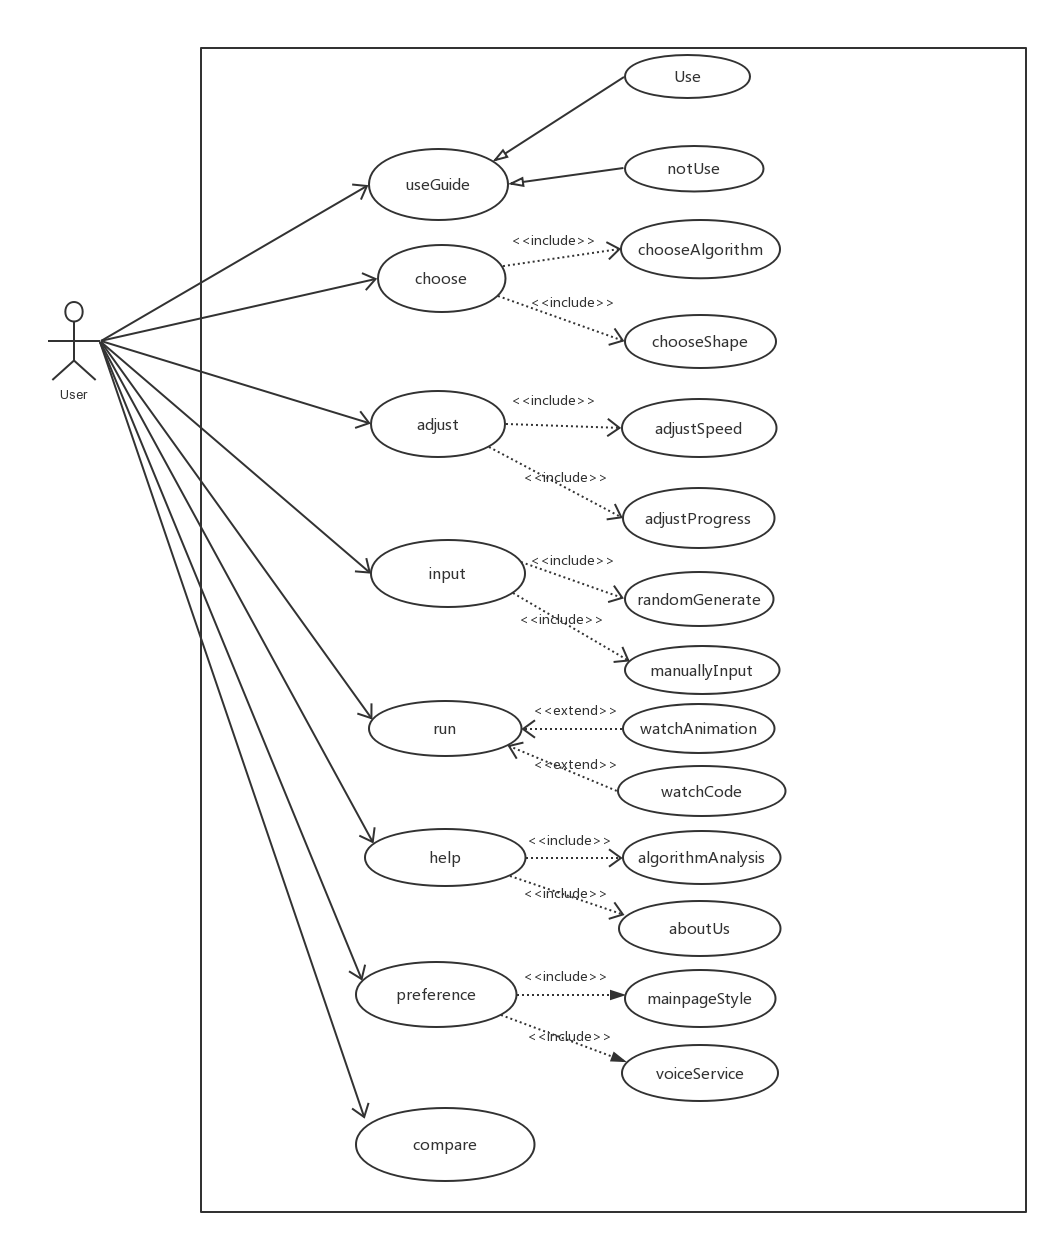
\includegraphics[width=.8\textwidth,height=.6\textwidth]{usecase.png}
\caption{Use case diagram}
\label{usecase}
\end{figure}
According to Wegmann and Genilloud(2000),  use case diagram is used to represent functions of the system and the intent of the diagram is to capture the roles of each participation to an action. From the figure \ref{usecase}, it can be seen that the user`s every action is captured to display in the picture, and each action extend to different functions, which clearly shows use cases of user and the functions corresponding to use case.
\subsubsection{Sequence diagram}
\begin{figure}[htbp]
\centering
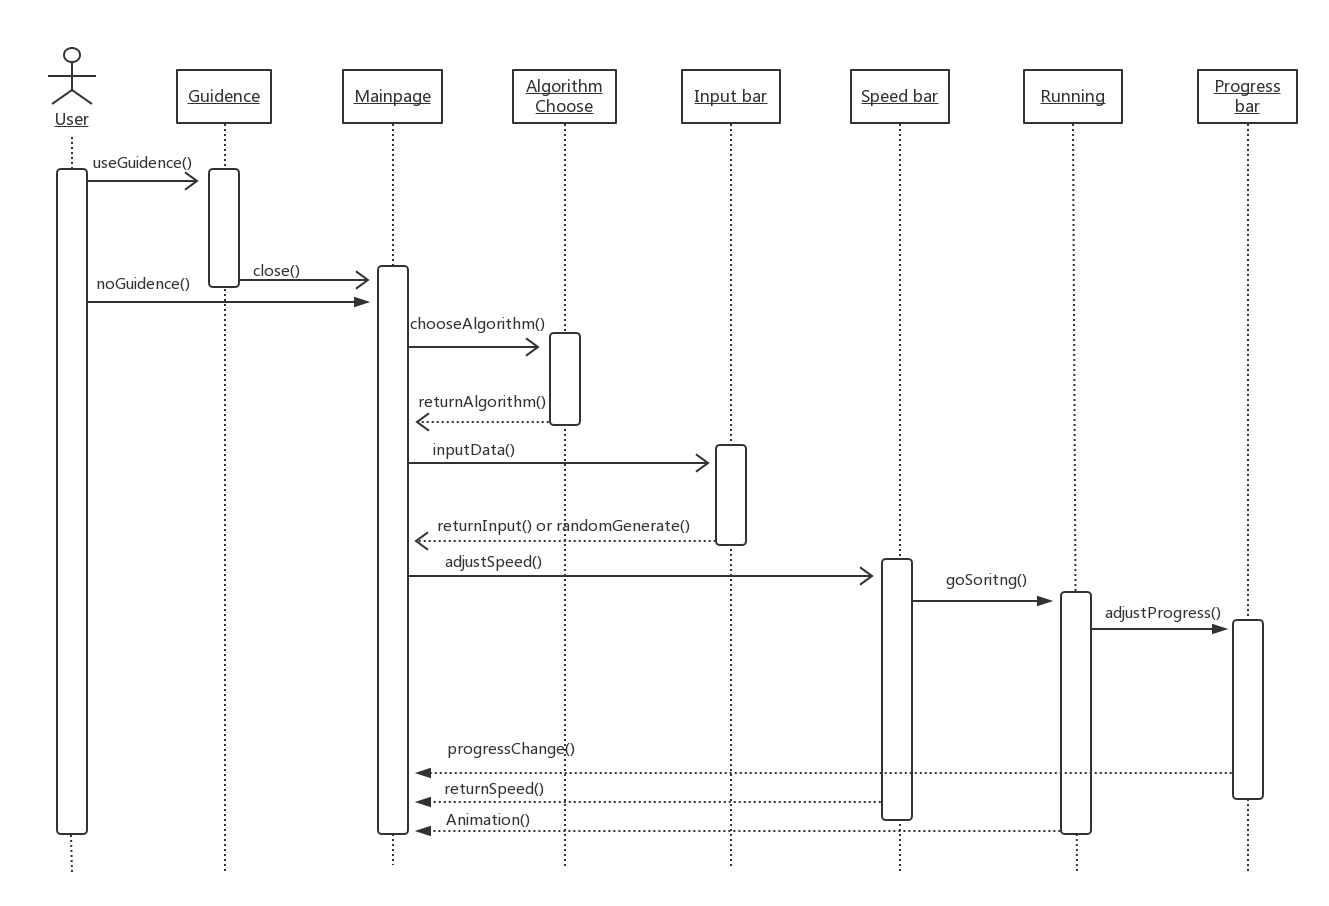
\includegraphics[width=.8\textwidth]{sequence.png}
\caption{Sequence diagram}
\label{sequence}
\end{figure}
Bell (2004) claims that sequence diagram primarily shows the interactions between objects in the sequential order that those events occur. The figure \ref{sequence} above shows the sequence of events happening when user have used all the functions and click running button at last. The sequence diagram clearly describes the timeline of events happening and the interactions among obejcts.

\subsection{Key Implementation Decision} 
\subsubsection{Programming languages}
The programming language is the basic part of the software. This part will depend the software using in which Operating System(OS) and the difficulty of the coding progress. As modern university teachers and students using both Windows and MacOS, so Java is a perfect choice because Java is a coding language which can be used in most of the operating systems. Another reason of using Java is that Java is the most popular programming language in the world and has a huge amount of open source libraries to make the software better. For the Graphical User Interface(GUI) part, firstly we decided to use swing, but we found JavaFX, a better GUI library which is intended to replace Swing as the basic GUI library for JavaSE. By using JavaFX, we used the web language (HTML, CSS and JavaScript) indirectly, this could help us to write a web app efficiently if we want to.

--- Optional

Writing and web app could solve the operating system problems because web app is showing its contents in the web browsers and almost all the equipments have the function of using a web browser.

\subsubsection{Operating systems}
The operating system(OS) is an important part of the software, it influences a lot to users using different operating systems. In nowadays university, though most students and teachers using Windows, the MacOS users also take up a big part. So the software should run in most of the operating systems, people should run the software where ever they want.

--- Optional

The software can be used in Android and IOS operating systems so that people can learning and watching algorithm animations on the phone in anywhere.

\subsubsection{Computers}
Nowadays, with the development of science and technology, more and more devices have become a necessity of life, such as mobile phone, tablet, laptop and desktop. Our target is to make a software which is 
convenient and easy for users to access, which means the software can be accessed in each kind of device, so that whenever people want to use the software, he can pick up any one of his devices around him and use it to access the software. In addition, the interface of software should be adapted to each kind of device to make users good use experience.

\subsubsection{Software in use}
\begin{enumerate}
\begin{figure}[htbp]
\centering
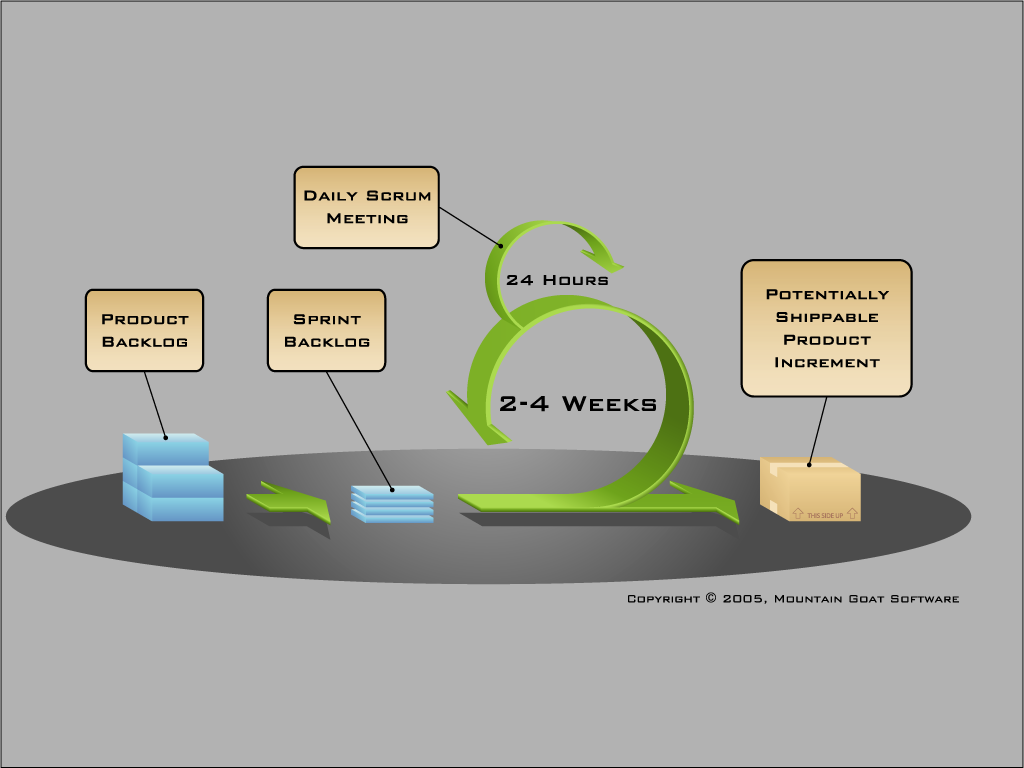
\includegraphics[width=.8\textwidth]{scrum.png}
\caption{Basic process of Scrum}
\label{scrum}
\end{figure}
	\item\textbf{Scrum: } Scrum is an agile software development methodology, which means it is an increment, iterative development process, and the development process consists of a number of short iteration cycles named sprint (the green curly arrow).  The basic process of scrum is described in the figure \ref{scrum}. In scrum, product backlog is a prioritized list of requirements used to manage product requirements. The Scrum team in a sprint selects the highest priority requirement from product backlog to develop. Then the selected requirements are analyzed and evaluated at the Scrum meeting to get a task list to be completed in the sprint called sprint backlog. When a sprint finished, the product increment is handed (Website, 2016). The process shows that scrum needs the team works as tight, focus on a single goal, understands the priorities and team memebers are clear about their roles (Rising and Janoff, 2000). It is necessary that our team works as the scrum team to develop our software. We set one sprint for a week, and finish a software requirement list as the product backlog, and everyday our team has a short meeting to discuss to-do-list, which will be released in Tower as sprint backlog. In each sprint, our team will have a formal meeting with supervisor to discuss the requirement selected and hand in product increment.
\begin{figure}[htbp]
\centering
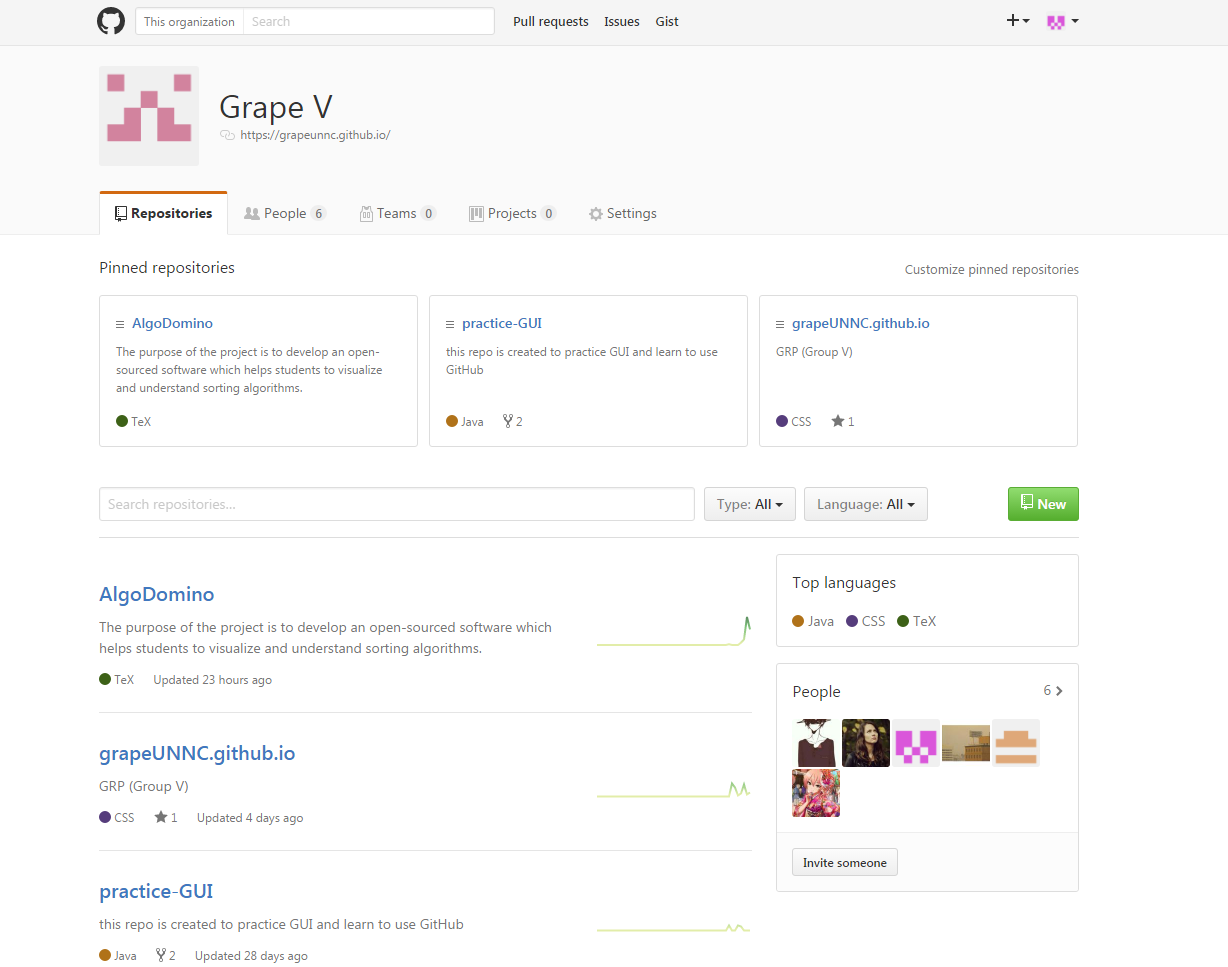
\includegraphics[width=.8\textwidth]{github.png}
\caption{Github page}
\label{github}
\end{figure}
	\item \textbf{Github: } As it is known, Git is an excellent distributed version control system, which can keep the history of a file set, and can roll back the file to another state (History). GitHub is a git based web collaboration community, it can not only work as Git to keep the history of a file and roll back the file state, but also have a variety of mechanisms for everyone to work together to contribute to the project. In addition, Github integrates lots of social features which make user`s information and activities visible across open source software projects (Dabbish el al, 2012). Our group decides to use Github as a basic tool to develop the software,  so that we can upload the software project to one repository where everyone can access and work on it, control the project version in case confict happens, and search some useful open resource distributed in Github. The link is {https://github.com/}.
\begin{figure}[htbp]
\centering
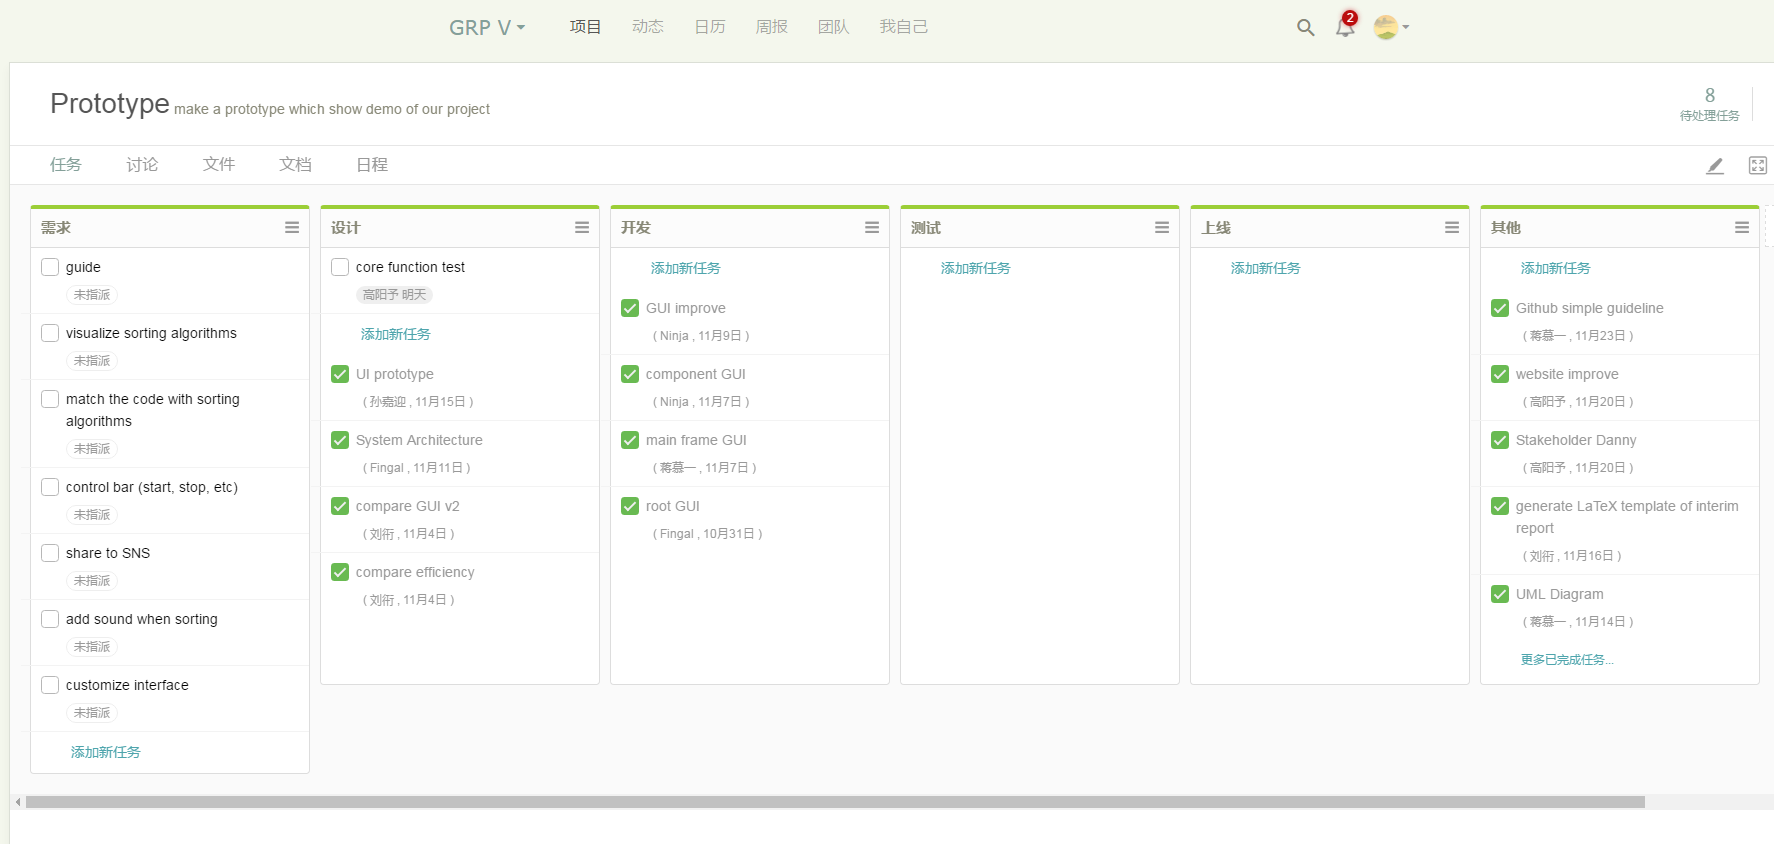
\includegraphics[width=.8\textwidth]{tower.png}
\caption{Tower page}
\label{tower}
\end{figure}
	\item \textbf{Tower: } Tower is an Agile development based team collaboration tools, and it can be used for Scrum to release to-do-list in each sprint. It's like an online office where you can quickly process tasks, conduct discussions, review project progress, and work with your team at any time. According to Cockburn and Highsmith (2001), agile development reduces the cost of exchanging information in a team and improves the team`s amicability---members` sense of community. These points are perfectly implemented in Tower. For instance, all the tasks are displayed  in the panel, and team members can access all the tasks to know about the details and progress, which is easy to exchange information, morever, when a task is finished or assigned, every team member will be reminded, which improves the sense of community. It is obvious that Tower can help a lot to develop the software, so we use it as our team collaboration tools.The link is {https://tower.im/} 
	\item \textbf{LaTex: } Oetiker (2010) claims that LaTex is a Tex based typesetting system. It is suitable for the production of high printing quality of science and technology and mathematics, and it also applies to all other types of documents that are generated from a simple letter to a complete book. And Oetiker (2010) also says "LaTeX is a macro package which enables authors to typeset and print their work at the highest typographical quality, using a professional layout." According to Oetiker`s points, the most important features Latex has is to print works at high quality, which is a necessary feature to be used in our software report. So we decide to use LaTex to edit our interim report and final report, to make them more academic and higher quality.
	\item \textbf{SceneBuilder JavaFX: } According to Jackson (2010), SceneBuilder JavaFX provides a visual layout environment that allows to quickly design the user interface for JavaFX applications (UI) without having to write any code. It allows a graphical interface (GUI) control to simply drag and drop to a JavaFX scene. When you create a user interface layout, FXML layout code will be automatically generated. SceneBuilder JavaFX provides a simple and intuitive user interface that can help developers quickly create an interactive application prototype that connects GUI controls to the application logic. It is efficient for us to use SceneBuilder JavaFX to design the high-fidelity prototype of  the software.
\end{enumerate}
\clearpage
\section{Implementation}
\subsection{Main Frame}
% Ninja progess
For the main frame of the sorting algorithm animation, the interface is divided into 5 parts. Each of these 5 parts is not independent. 
\begin{enumerate}
   \item The main part is the animation. This part include several data and the geometric figure generated by them. When program is running, they will move on the basis of algorithm codes. The place changing can easily explain how the selected algorithm works. 
   \item The second part, which is under the animation, is control function. It contains 5 functional buttons and they work together to control the animation of algorithm. The first button on the left-up corner of this part is the “play-stop” button. When the “stop” button is click, the animation will freeze at the present step. Then the “stop” button will become the “paly” button. The animation will not continue the rest step until the “play” button is clicked. 
   \item The controller on the right side of the “play-stop” button is progress line. User can drug the button on the line to control the progress of animation. The animation will stop at differential steps with differential positions. 
   \item The button at the lower left corner is the speed bar. The speed input box is on the right side. These two controllers is used to control the speed of animation. User can change the speed of figure moving through drugging the control line or inputting an integer level from 1 to 10. 
   \item The last button at the lower right corner in this part is shape chosen box. User can choose or change the shape of figures in this choose box. Several figures such as rectangle, triangle and circle are provided for users. This function will not influence the process of algorithm code running. 

\end{enumerate}


% ------------------------------------------------------------------------------
% Implementation     Zhe REN, Jiaying SUN, Yangyu GAO
% -----------------------------------------------------------------------------
This section introduces the basic prototype and give a particular introduction of this software. More specifically, prototypes have been done including toolbar, sorting window and comparison window. The software is based on response type so that each sectional window can change its size. Response type make the software more reasonable.

\subsection{Main Page}
\begin{enumerate}
\item  Main frame \\For the main frame of the sorting algorithm animation, the interface is divided into 5 parts. Each of these 5 parts is not independent. The main part is the animation. This part include several data and the geometric figure generated by them. When program is running, they will move on the basis of algorithm codes. The place changing can easily explain how the selected algorithm works. The second part, which is under the animation, is control function. It contains 5 functional buttons and they work together to control the animation of algorithm. The first button on the left-up corner of this part is the “play-stop” button. When the “stop” button is click, the animation will freeze at the present step. Then the “stop” button will become the “paly” button. The animation will not continue the rest step until the “play” button is clicked. The controller on the right side of the “play-stop” button is progress line. User can drug the button on the line to control the progress of animation. The animation will stop at differential steps with differential positions. The button at the lower left corner is the speed bar. The speed input box is on the right side. These two controllers is used to control the speed of animation. User can change the speed of figure moving through drugging the control line or inputting an integer level from 1 to 10. The last button at the lower right corner in this part is shape chosen box. User can choose or change the shape of figures in this choose box. Several figures such as rectangle, triangle and circle are provided for users. This function will not influence the process of algorithm code running. 

\item Algorithm Setting Block \\
Sorting algorithms are able to selected in a scrollbar. The sequence of sorting algorithms is Bubble Sort, Selection Sort, Insertion Sort, Merge Sort, Quick Sort, Heap Sort, Bucket Sort according to the difficulties increasing. The default algorithm is Bubble Sort. When the algorithm selected, users can click the “Start” button to start. \\
Users can not able to change the input and the number of inputs considering two aspects. On one hand, it makes no sense if users specify a serial of same numbers or increasing numbers. One the other hand, considering the users experience, if user input too many numbers, it will affect user experience due to long waiting time. 

\item Comment Block \\It connects to the amination and running code block. The comment shows the explanation of running code concurrently. 

\item Running Code Block \\It connects to the amination and comment block. It shows the Java code running according the step of animation.
\end{enumerate}


\subsection{Comparing Part}

Comparing sorting algorithms is another section of the software. In the right hand side there is a selection part where users can select which two algorithms to compare. After choosing the algorithms, the main part change to two single parts which locate in left and right side. Each part is an independent part which has its own animation process.\\

In each of the animation part, the total time will show in the top of the window, below the sorting graph, it shows the name of the sorting algorithm.\\

Two algorithms both have the same default input and start in the same time after pressing the ‘Start’ button. In the right hand side, below the algorithm choosing window there is a part which can show the complexity of the algorithms which is comparing in the main window. After the comparing process, the efficiency line chart of different sorting algorithms in a clear pattern.\\

— Optional
The main requirement only provides two algorithms to compare, so the comparison windows maybe larger. Users can choose how many algorithms they want to compare. The right hand side windows’ function should also change because of the number of windows become larger.
\clearpage

% ------------------------------------------------------------------------------
% Progress Report    Zhefeng ZHOU
% -----------------------------------------------------------------------------
\section{Progress Report}
This section mainly covers 3 parts, progress we made, problems we met and our time plan. The first subsection summarizes the progress we made so far, the second subsection discusses some problems encountered, including both technical and management issues, and the third subsection talks about the future time plan of the project. \\
Reference Example\cite{Debray:2000:CTC:349214.349233}

\subsection{Progress to date}
% FINGAL progess
As mentioned in the previous sections, a portion of this project is dedicated to research and investigation in order to elicit the requirements, best technologies for the job and conduct some feasibility studies on past existing or novel solutions that solve some part(s) or all of the problem. It is therefore important to emphasize the role these play and their sizable contribution to the progress made. The progress thus far is as follows:
\begin{enumerate}
	\item \textbf{Project Website: } The project website is using Jekyll and is free hosting in GitHub Pages, which link is \url{grapeUNNC.github.io}. The website provide basic introduction of the project and the team role.
	\item \textbf{Requirements Specification: }The Functional and Non-Functional requirements specifications were determined and enumerated. The elicitation of these specifications had an effect on the time frame of the project such that it necessarily had to be adjusted to account for further research and implementation components.
	\item \textbf{System Design: }Given the requirements of the system, it was necessary to formulate a design which would be followed in the implementation of the system. This also added to the direction of the project so that the Feasibility Study and Prototyping stages were better informed with respect to suitability.
	\item \textbf{Feasible Study: }An evaluation of current novel and existing technologies and systems is made in order to best determine the extent to which they solved the problem(s) outlined in the Specifications. A decision was also made on which of these would be used in order to progress with this project and solve the problems outlined therein.
	\item \textbf{Prototype: }Basic prototyping was done following the designs of the system to trial run some of the technologies chosen for parts of the project and evaluate the scope, direction and projections of the project.
\end{enumerate}
\subsection{Problems encountered}
% FINGAL problems
\subsection{Time plans for the next half}
The second half of the cycle will be composed largely of implementation, testing and debugging steps in order to realize the design.
% INCLUDE GANTT CHART HERE

\clearpage

% ------------------------------------------------------------------------------
% Appendices
% ------------------------------------------------------------------------------
\section{Appendices}
\clearpage

% ------------------------------------------------------------------------------
% Bibliography
% ------------------------------------------------------------------------------
\bibliographystyle{plain}
\bibliography{InterimReport_Grape}

% ------------------------------------------------------------------------------
% End document
% ------------------------------------------------------------------------------
\end{document}




